\scanpage{72}
% archive foliation: 71
% Small lower-right archival mark: JSVO (uncertain).
\uline{Th.} \textcircled{I} Soit $X$ une courbe analytique \uline{régulière},
$\deleted{\unsure{\mathcal{P}}}\inserted{\mathcal{E}_X}$ ($\mathcal{P}_X$) le
faisceau des applications étales d'ouverts de $X$ dans
$\unsure{\underline{E}^{1}|\underline{A}^{1}}(\mathbb{C})$
($\mathbb{P}^{1}(\mathbb{C})$). Il existe un morphisme
\[
G:\mathcal{E}_X\times\mathcal{E}_X\longrightarrow
\underline{\omega}_{X/\mathbb{C}}^{\otimes2}
\qquad
(\underline{\omega}_{X/\mathbb{C}}=\underline{\Omega}^{1}_{X/\mathbb{C}})
\]
ayant les propriétés suivantes

a) $G$ est un op. différentiel (pas néc. linéaire), i.e. en
termes d'un uniformisant local $t$ \inserted{(défini sur un ouvert $U$)} on a
\[
G(f,g)=R(f,f',\ldots,f^{(n)},g,g',\ldots,g^{(n)})dt^2
\]
$R$ est une fonction rationnelle en $2n$ variables, à
coefficients dans $\Gamma(\unsure{X|U},\mathcal{O}_U)$.
\inserted{où $R=P/Q$, $P$ et $Q$ polynômes.}
De plus, \deleted{le dénominateur}
$Q$ non identiquement nul, \deleted{\unsure{si on substitue}} ce qui implique
\deleted{est tel qu'il n'a pas des \deleted{pôles} zéros}
que $Q(f,\unsure{g'|f'},\ldots,f^{(n)};g,g',\ldots,g^{(n)})$ n'est pas identiquement
\deleted{\unsure{quel que} $f$ et $g$, \unsure{comme} \unsure{ci}}
nul, on suppose que $Q$ ne s'annule identiquement pour
aucun $f$ et $g$ où $f$ et $g$ non loc. constants ni l'un
ni l'autre, et que $P(f,\ldots,g,\ldots)/Q(f,\ldots,g,\ldots)$ n'a
\deleted{pas} des pôles qu'aux pt où $f',g'$ ont des zéros.

[On doit pouvoir montrer que, si on prend $P,Q$
premiers entre eux, on aura \inserted{\unsure{pour facteurs}}
$Q=f'{}^p g'{}^q$, donc
\[
G(f,g)=\frac{1}{f'{}^p g'{}^q}
P(f,f',\ldots,f^{(n)};g,g',\ldots,g^{(n)})
\]
]

b) $G(f,g)+G(g,h)=G(f,h)$

c)
\[
\begin{aligned}
G(f,ag)&=G(f,g)\deleted{\unsure{=G(f,1/g)}}
&&\inserted{a\in\mathbb{C}^{*}}\quad
\deleted{\text{si }a\in\mathbb{C}^{*},\ b\in\mathbb{C}}\\
&&&\deleted{(\text{et }g)}\\
G(f,g+b)&=G(f,g)&&b\in\mathbb{C}\\
G(f,1/g)&=G(f,g)&&\text{si }g\text{ sans zéros}
\end{aligned}
\]

d) \deleted{\unsure{Pour $f$ fixé}} Si $G(f,g)=0$ et $f,g$ coïncident à l'ordre $2$
en un point $x\in X$ (\unsure{i.e.}, $f,g\in\Gamma(U,\underline{\mathcal{O}}_U)$)
alors $f=g$ si $U$ connexe.

Deux tels morphismes $G'$ et $G$ sont liés par
\[
G'=\varphi G,\quad\text{avec }\varphi\in\Gamma(X,\underline{\mathcal{O}}_X^{*})
\]

\margin{\uline{NB} c) implique que $G$ se descend en
$\mathcal{P}_X\times\mathcal{P}_X\longrightarrow\underline{\omega}_X^{\otimes2}$,
\deleted{\unsure{et la factorise en}}
$H\backslash\mathcal{P}_X\times {}_H\mathcal{P}_X\longrightarrow
\underline{\omega}_X^{\otimes2}$, où $H=\unsure{GP(1,\mathbb{C})|GA(1,\mathbb{C})}$.
b) donne la relation analogue pour ${}_H\mathcal{P}_X$,
\diagram{\begin{tikzcd}
H\backslash\mathcal{P}_X \arrow[r,"c"] & \mathcal{T}
\end{tikzcd}}
où $G(f,g)=c(f)-c(g)$, \unsure{alors}
d'où \unsure{torseur} $\mathcal{T}_X$ \unsure{et|est}
de groupe $\unsure{\underline{\omega}_X^{\otimes2}}$.}

\margin{d) $H\backslash\mathcal{P}_X\longrightarrow\mathcal{T}_X$ est mono,
et e) que c'est épi.}
\figure{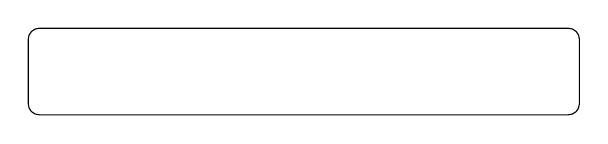
\begin{tikzpicture}
\draw[rounded corners] (0,0) rectangle (7,1.1);
\end{tikzpicture}}

\margin{e) Si $f\in\Gamma(U,\mathcal{E}_U)$, le morphisme
$g\mapsto G(f,g)$ de $\mathcal{E}_U$ dans $\underline{\omega}_U^{\otimes2}$ est
un épi.}

\textcircled{II} Si, au lieu de prendre $X$ fixe, on prend $X$ variable,
avec \unsure{morphismes|compatibilités} étales entre des $X$, on a
$=$ résultat, et l'indétermination sera
\[
G'=cG\qquad c\in\mathbb{C}^{*}\quad !
\]

\margin{Ici, au lieu des \unsure{la condition|conditions} d) e)
il suffit de supposer d)
\deleted{\unsure{de groupe} \unsure{additif|trivial}}.}
\figure{\begin{tikzpicture}
\draw[rounded corners] (0,0) rectangle (4.8,2.2);
\draw (0.2,2.15) .. controls (-0.3,2.6) and (-0.5,2.3) .. (-0.3,2.1);
\end{tikzpicture}}

